\documentclass[%
	11pt,
	a4paper,
	utf8,
	%twocolumn
		]{article}	

\usepackage{style_packages/podvoyskiy_article_extended}


\begin{document}
\title{Сборник заметок\\по использованию Kubernetes в контексте машинного обучения}

\author{}

\date{}
\maketitle

\thispagestyle{fancy}

\tableofcontents


\section{Основные термины}

\noindent\emph{под} (pod) -- группа \emph{контейнеров} (один или несколько); минимальная сущность, управляемая Kubernetes; у всех контейнеров внутри одного пода общие network, IPC, UTS, PID*, namespace; pod нельзя делить между узлами кластера \pic{fig:pod}; на \pic{fig:podpatterns} приведены основные паттерны использования подов

\begin{figure}[h]
	\centering
	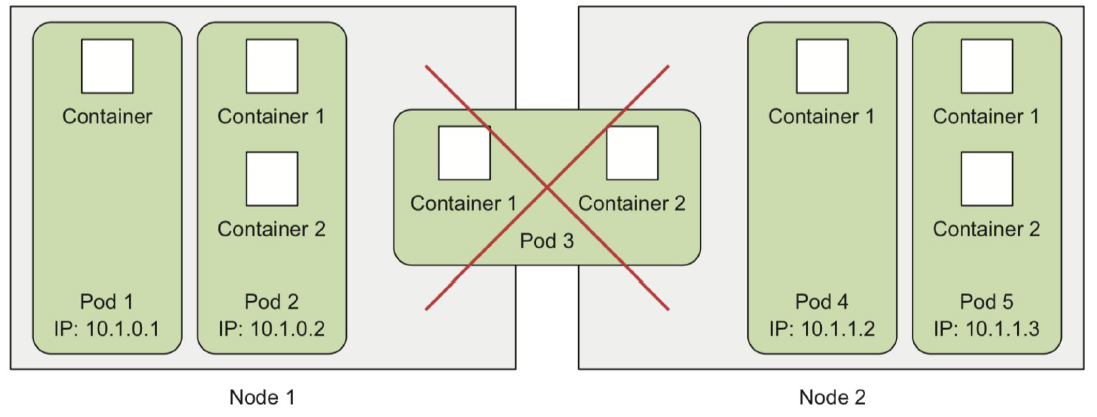
\includegraphics[scale=0.55]{figures/pod.png}
	\caption{ Иллюстрация концепции подов }\label{fig:pod}
\end{figure}

\begin{figure}[h]
	\centering
	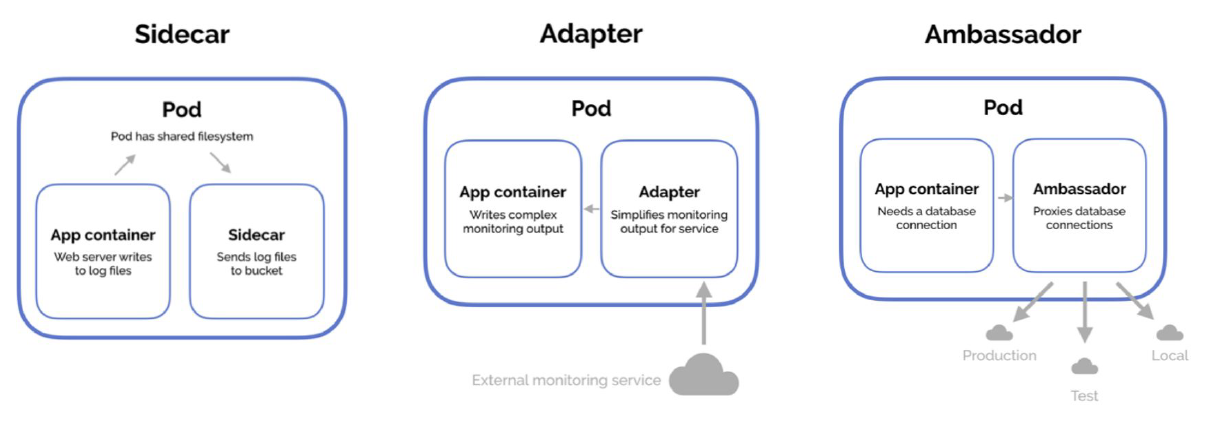
\includegraphics[scale=0.55]{figures/podpatterns.png}
	\caption{ Паттерны использования подов }\label{fig:podpatterns}
\end{figure}


\section{Общие замечания}

Для небольших проектов из нескольких контейнеров удобнее использовать оркестратор Nomad \url{https://www.nomadproject.io/}.


\section{Начало работы в Kubernetes с помощью Minikube}

Для работы с Kubernetes система должна поддреживать виртуализацию. На MacOS X это можно проверить так
\begin{lstlisting}[
style = bash,
numbers = none
]
sysctl -a | grep machdep.cpu.features | grep VMX
\end{lstlisting}

Если возвращается непустой результат, то можно продолжать. Теперь требуется установить гипервизор, например, VirtualBox \url{https://www.virtualbox.org/wiki/Downloads}.

Далее требуется установить \texttt{minikube}. На Mac OS X это можно сделать с помощью менеджера \texttt{brew}
\begin{lstlisting}[
style = bash,
numbers = none	
]
brew install minikube
\end{lstlisting}

\texttt{minikube} -- утилита командной строки для настройки и запуска \emph{одноузлового кластера Kubernetes} в виртуальной машине на \emph{локальном} компьютере. Этот вариант идеально подходит для первого знакомства с кластером под управлением Kubernetes и выполнения простых операций.

Проверка установки
\begin{lstlisting}[
style = bash,
numbers = none	
]
minikube start --vm-driver=virtualbox
minikube status
\end{lstlisting}

Если кластер запущен, то в выводе команды \texttt{minikube status} должно быть что-то вроде
\begin{lstlisting}[
style = bash,
numbers = none	
]
host: Running
kubelet: Running
apiserver: Running
kubeconfig: Configured
\end{lstlisting}

Вместе с \texttt{minikube} устанавливается и утилита \texttt{kubectl} для работы с полноценным кластером под управлением Kubernetes.

Можно посмотреть список запущенных в кластере подов (групп контейнеров) и нод
\begin{lstlisting}[
style = bash,
numbers = none	
]
kubectl get pods --all-namespaces
kubectl get nodes
\end{lstlisting}

Теперь можно запустить встроенный под \texttt{hello-minikube}. Для этого пода будет создан предварительно настроенный deployment
\begin{lstlisting}[
style = bash,
numbers = none	
]
kubectl run hello-minikube --image=gcr.io/google_containers/echoserver:1.4 --port=8080 # pod/hello-minikube created
\end{lstlisting}

Можно снова посмотреть на актуальные списки подов
\begin{lstlisting}[
style = bash,
numbers = none	
]
kubectl get pods
\end{lstlisting}

Удалить под и ноду
\begin{lstlisting}[
style = bash,
numbers = none	
]
kubectl delete pod hello-minikube
kubectl delete node minikube
\end{lstlisting}



% Источники в "Газовой промышленности" нумеруются по мере упоминания 
\begin{thebibliography}{99}\addcontentsline{toc}{section}{Список литературы}
	\bibitem{juba:2019}{ \emph{Джуба С.}, \emph{Волков А.} Изучаем PostgreSQL 10. -- М.: ДМК Пресс, 2019. -- 400 с.}
\end{thebibliography}

%\listoffigures\addcontentsline{toc}{section}{Список иллюстраций}

\lstlistoflistings\addcontentsline{toc}{section}{Список листингов}

\end{document}
